\expandafter\newcommand\csname dataRFmetrictab\endcsname{
\begin{table}[H]
\begin{tabular}
{| 
 p{\dimexpr0.2\textwidth-2\tabcolsep-\arrayrulewidth\relax}| 
 p{\dimexpr0.2\textwidth-2\tabcolsep-\arrayrulewidth\relax}| 
 p{\dimexpr0.2\textwidth-2\tabcolsep-\arrayrulewidth\relax}| 
 p{\dimexpr0.2\textwidth-2\tabcolsep-\arrayrulewidth\relax}| 
 p{\dimexpr0.2\textwidth-2\tabcolsep-\arrayrulewidth\relax}| 
}\hline 
\textbf{} &\textbf{f1-score} &\textbf{precision} &\textbf{recall} &\textbf{support} \\ \hline 
CANDIDATE &0.966 &0.986 &0.947 &76.0 \\ \hline 
CONFIRMED &0.989 &0.982 &0.996 &223.0 \\ \hline 
FALSE POSITIVE &0.991 &0.991 &0.991 &114.0 \\ \hline 
accuracy &0.985 &0.985 &0.985 &0.985 \\ \hline 
macro avg &0.982 &0.987 &0.978 &413.0 \\ \hline 
weighted avg &0.985 &0.986 &0.985 &413.0 \\ \hline 
\end{tabular} 
\end{table}
}
\begin{figure}[H]
                \begin{mdframed}[linecolor=green]
                \centering
                \begin{subfigure}{.49\textwidth}
                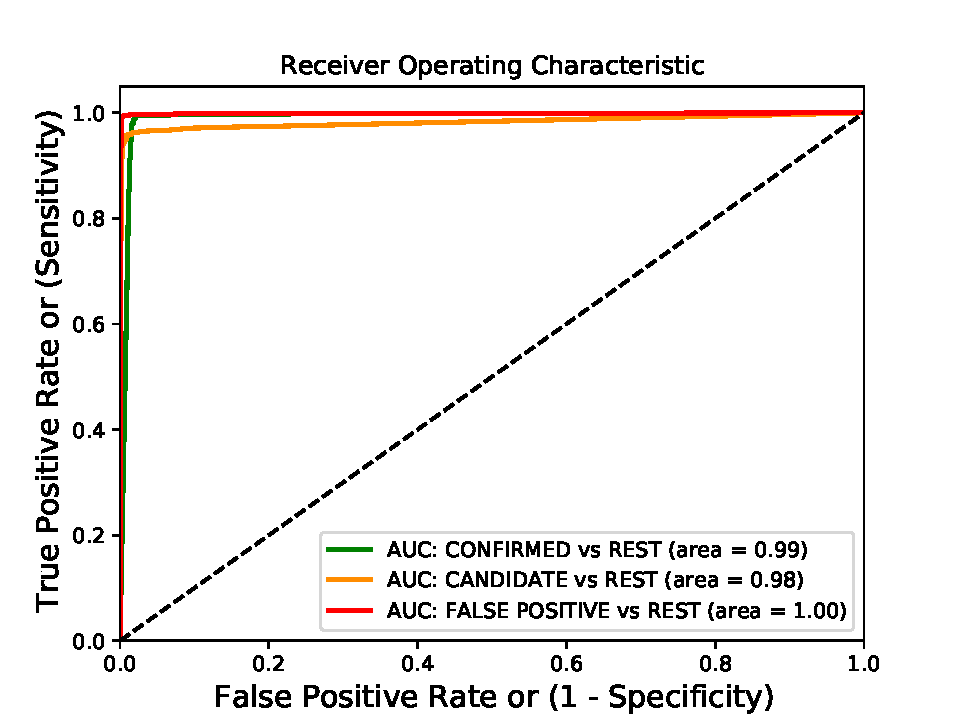
\includegraphics[width = 1\textwidth]{data/RF_overfit_roc.pdf}
                \end{subfigure}
                \begin{subfigure}{.49\textwidth}
                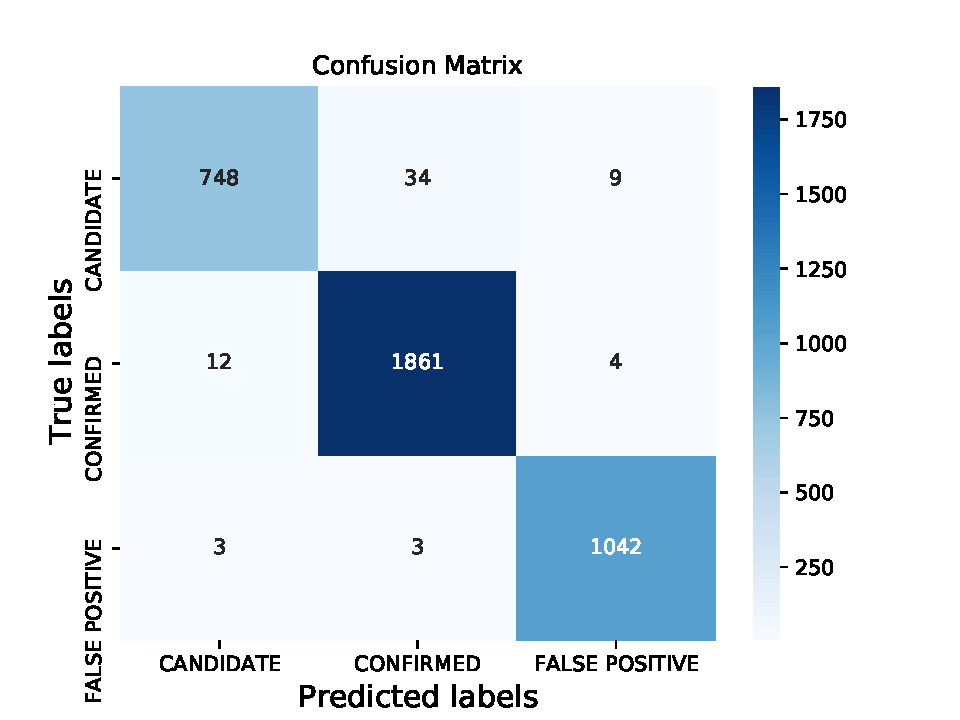
\includegraphics[width = 1\textwidth]{data/RF_overfit_cm.pdf}
                \end{subfigure}
                \begin{subfigure}{.49\textwidth}
                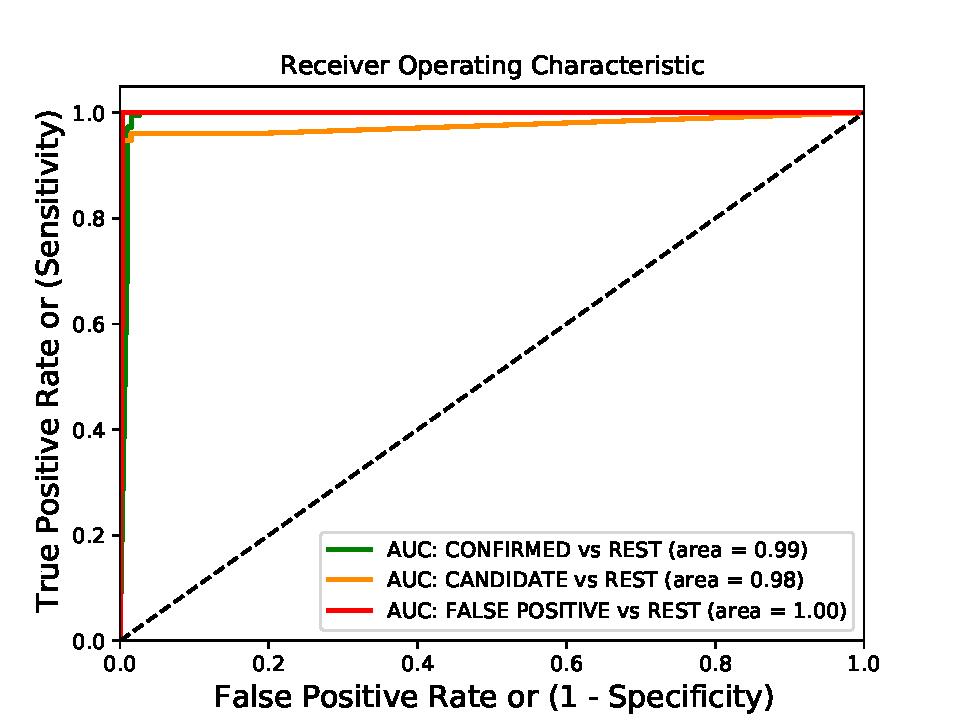
\includegraphics[width = 1\textwidth]{data/RF_roc.pdf}
                \end{subfigure}
                \begin{subfigure}{.49\textwidth}
                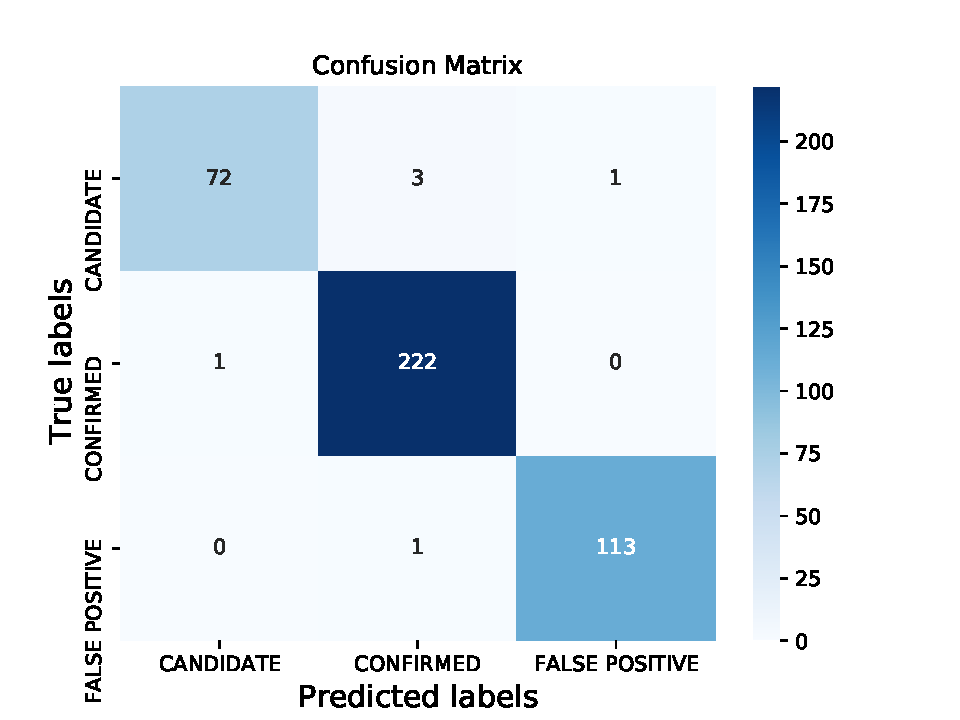
\includegraphics[width = 1\textwidth]{data/RF_cm.pdf}
                \end{subfigure}
                \begin{subfigure}{1\textwidth}
                \csname dataRFmetrictab\endcsname
                \end{subfigure}
                \caption{RF: Top Row: overfit test. Middle and bottom row test data}
                \label{fig:data/RF_roc}
                \end{mdframed}
                \end{figure}